\documentclass[border=6pt,tikz]{standalone}
\usepackage{amsmath,amssymb}
\usepackage{tikz}
\usetikzlibrary{arrows.meta,calc,decorations.pathreplacing,patterns,shapes.geometric,positioning,shadings,plotmarks}

\begin{document}
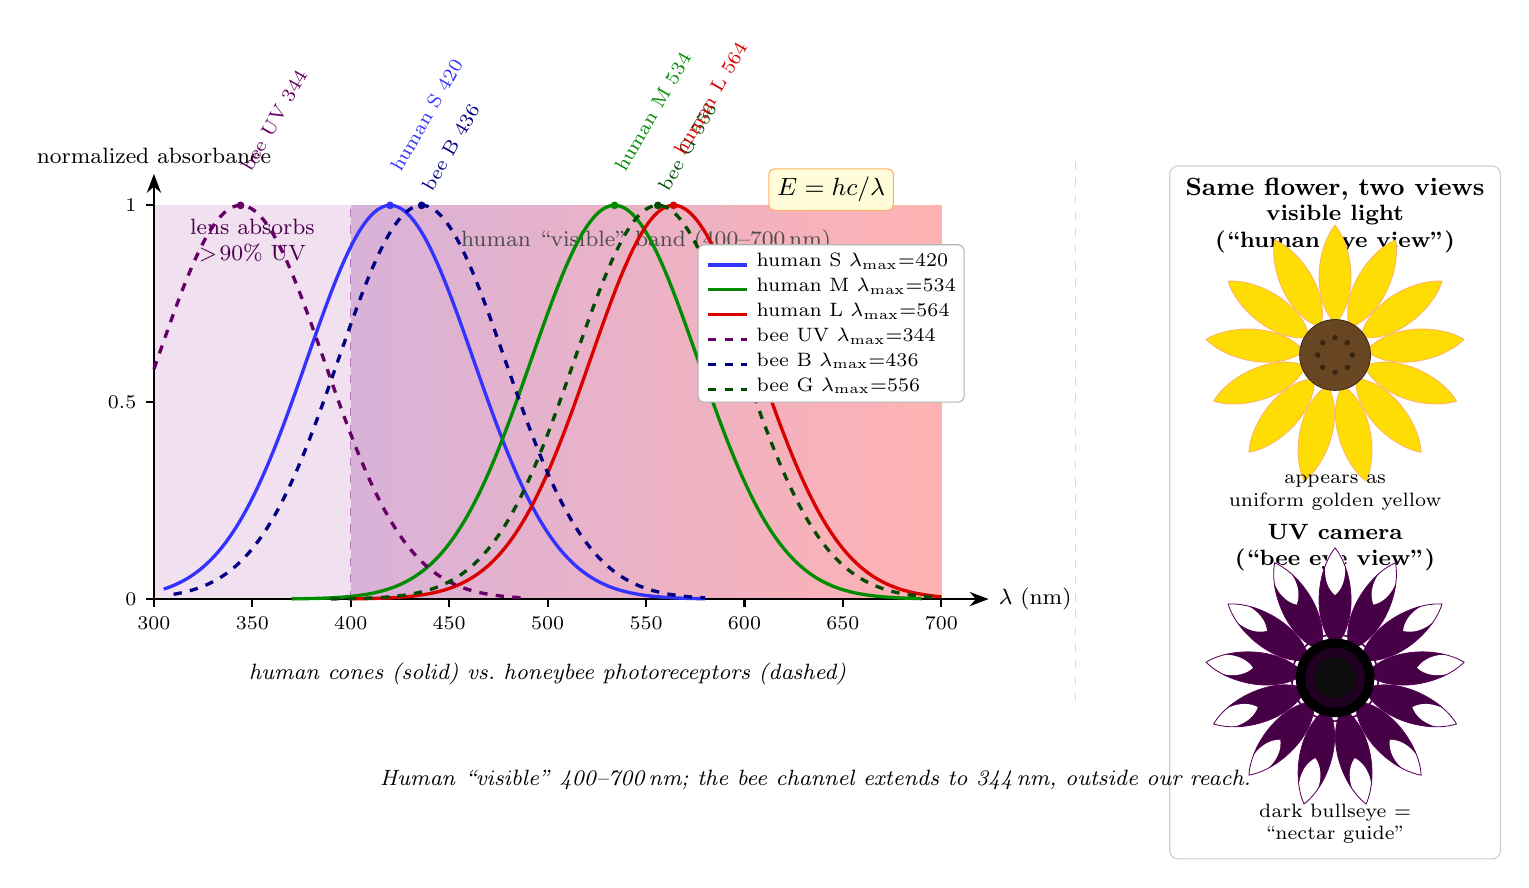
\begin{tikzpicture}[>={Stealth[length=2.4mm]},font=\small]

% ============================================================
% LEFT PANEL: Absorption spectra comparison
% x: 300..700 nm -> 0..10 cm;  y: 0..1 -> 0..5 cm
% ============================================================
\def\xn#1{({(#1-300)/40})}

% Rainbow band for 400..700 nm (human visible)
\shade[left color=violet!30,right color=red!30]
  ({(400-300)/40},0) rectangle ({(700-300)/40},5);

% UV band 300..400 nm (blocked by lens)
\fill[violet!12] (0,0) rectangle ({(400-300)/40},5);
\draw[violet!55,dashed] ({(400-300)/40},0) -- ({(400-300)/40},5);

\node[font=\footnotesize,violet!60!black,align=center]
  at ({(350-300)/40},4.55) {lens absorbs\\$>\!90\%$ UV};
\node[font=\footnotesize,black!70]
  at ({(550-300)/40},4.55) {human ``visible'' band (400--700\,nm)};

% Axes
\draw[->,thick] (-0.05,0) -- (10.6,0) node[right,font=\footnotesize]{$\lambda$ (nm)};
\draw[->,thick] (0,-0.05) -- (0,5.4) node[above,font=\footnotesize]{normalized absorbance};

% X ticks
\foreach \nm in {300,350,400,450,500,550,600,650,700}{
  \draw[thick] ({(\nm-300)/40},0) -- ({(\nm-300)/40},-0.1);
  \node[below,font=\scriptsize] at ({(\nm-300)/40},-0.1) {\nm};
}
% Y ticks
\foreach \y/\lab in {0/0,0.5/0.5,1/1}{
  \draw[thick] (0,{\y*5}) -- (-0.1,{\y*5});
  \node[left,font=\scriptsize] at (-0.1,{\y*5}) {\lab};
}

% Gaussian bell curves: A(nm) = exp(-((nm-mu)/sigma)^2), sigma ~ 60 for FWHM ~ 100 nm
% amplitude * 5 so peak touches y=5 (= normalized 1)

% HUMAN cones: solid, 1.2pt
\draw[blue!80,line width=1.2pt,smooth,samples=120,domain=305:580]
  plot ({(\x-300)/40},{5*exp(-((\x-420)/60)^2)});
\draw[green!55!black,line width=1.2pt,smooth,samples=120,domain=370:690]
  plot ({(\x-300)/40},{5*exp(-((\x-534)/60)^2)});
\draw[red!85!black,line width=1.2pt,smooth,samples=120,domain=400:700]
  plot ({(\x-300)/40},{5*exp(-((\x-564)/60)^2)});

% BEE receptors: dashed, 1.2pt, darker hues
\draw[violet!80!black,line width=1.2pt,dashed,smooth,samples=120,domain=300:490]
  plot ({(\x-300)/40},{5*exp(-((\x-344)/60)^2)});
\draw[blue!50!black,line width=1.2pt,dashed,smooth,samples=120,domain=310:580]
  plot ({(\x-300)/40},{5*exp(-((\x-436)/60)^2)});
\draw[green!30!black,line width=1.2pt,dashed,smooth,samples=120,domain=390:700]
  plot ({(\x-300)/40},{5*exp(-((\x-556)/60)^2)});

% Peak markers (dots at top of each curve) and labels
\foreach \mu/\col/\lab/\yoff in {%
  344/violet!80!black/{bee UV 344}/0.35,
  420/blue!80/{human S 420}/0.35,
  436/blue!50!black/{bee B 436}/0.10,
  534/green!55!black/{human M 534}/0.35,
  556/green!30!black/{bee G 556}/0.10,
  564/red!85!black/{human L 564}/0.55%
}{
  \fill[\col] ({(\mu-300)/40},5) circle (1.4pt);
  \node[\col,font=\scriptsize,rotate=60,anchor=west]
    at ({(\mu-300)/40},{5+\yoff}) {\lab};
}

% Legend box (inside upper-right area, below 650)
\node[draw=gray!60,rounded corners=2pt,fill=white,align=left,font=\scriptsize,inner sep=3pt]
  at (8.6,3.5)
  {\tikz\draw[blue!80,line width=1.2pt] (0,0) -- (0.5,0);\ human S $\lambda_{\max}{=}420$\\[1pt]
   \tikz\draw[green!55!black,line width=1.2pt] (0,0) -- (0.5,0);\ human M $\lambda_{\max}{=}534$\\[1pt]
   \tikz\draw[red!85!black,line width=1.2pt] (0,0) -- (0.5,0);\ human L $\lambda_{\max}{=}564$\\[1pt]
   \tikz\draw[violet!80!black,line width=1.2pt,dashed] (0,0) -- (0.5,0);\ bee UV $\lambda_{\max}{=}344$\\[1pt]
   \tikz\draw[blue!50!black,line width=1.2pt,dashed] (0,0) -- (0.5,0);\ bee B $\lambda_{\max}{=}436$\\[1pt]
   \tikz\draw[green!30!black,line width=1.2pt,dashed] (0,0) -- (0.5,0);\ bee G $\lambda_{\max}{=}556$};

% Energy formula box
\node[draw=orange!60,rounded corners=2pt,fill=yellow!15,font=\small,inner sep=3pt]
  at (8.6,5.2) {$E=hc/\lambda$};

% Left panel caption
\node[font=\footnotesize\itshape,align=center] at (5,-0.95)
  {human cones (solid) vs.\ honeybee photoreceptors (dashed)};

% ============================================================
% RIGHT PANEL: Two flowers
% ============================================================
\begin{scope}[xshift=12.6cm,yshift=0cm]

% Title
\node[font=\small\bfseries] at (2.4,5.2) {Same flower, two views};

% --- FLOWER 1 (top): visible-light view, uniform yellow ---
\node[font=\footnotesize\bfseries,align=center] at (2.4,4.7)
  {visible light\\(``human eye view'')};

% Petals (13 petals)
\begin{scope}[shift={(2.4,3.1)}]
  \foreach \a in {0,27.7,55.4,83.1,110.8,138.5,166.2,193.8,221.5,249.2,276.9,304.6,332.3}{
    \begin{scope}[rotate=\a]
      \fill[yellow!80!orange]
        (0,0.4) .. controls (0.3,0.7) and (0.24,1.35) .. (0,1.65)
        .. controls (-0.24,1.35) and (-0.3,0.7) .. (0,0.4) -- cycle;
      \draw[orange!60,line width=0.3pt]
        (0,0.4) .. controls (0.3,0.7) and (0.24,1.35) .. (0,1.65)
        .. controls (-0.24,1.35) and (-0.3,0.7) .. (0,0.4) -- cycle;
    \end{scope}
  }
  % center disc (brown)
  \fill[brown!55!black] (0,0) circle (0.45);
  \draw[brown!30!black,line width=0.3pt] (0,0) circle (0.45);
  \foreach \a in {0,45,90,135,180,225,270,315}{
    \fill[brown!30!black] (\a:0.22) circle (0.035);
  }
\end{scope}

\node[font=\scriptsize,align=center] at (2.4,1.35)
  {appears as\\uniform golden yellow};

% --- FLOWER 2 (bottom): UV view, dark bullseye + glowing tips ---
\node[font=\footnotesize\bfseries,align=center] at (2.4,0.65)
  {UV camera\\(``bee eye view'')};

\begin{scope}[shift={(2.4,-1)}]
  \foreach \a in {0,27.7,55.4,83.1,110.8,138.5,166.2,193.8,221.5,249.2,276.9,304.6,332.3}{
    \begin{scope}[rotate=\a]
      % dark base petal (UV-absorbing)
      \fill[violet!55!black]
        (0,0.4) .. controls (0.3,0.7) and (0.24,1.35) .. (0,1.65)
        .. controls (-0.24,1.35) and (-0.3,0.7) .. (0,0.4) -- cycle;
      % bright tip (UV reflective)
      \fill[white]
        (0,1.05) .. controls (0.18,1.2) and (0.16,1.55) .. (0,1.65)
        .. controls (-0.16,1.55) and (-0.18,1.2) .. (0,1.05) -- cycle;
      \draw[violet!70!black,line width=0.3pt]
        (0,0.4) .. controls (0.3,0.7) and (0.24,1.35) .. (0,1.65)
        .. controls (-0.24,1.35) and (-0.3,0.7) .. (0,0.4) -- cycle;
    \end{scope}
  }
  % Dark UV bullseye (radius ~0.5 for ~30% of flower diameter ~3.3)
  \fill[black] (0,0) circle (0.5);
  \fill[violet!25!black] (0,0) circle (0.38);
  \fill[black!95] (0,0) circle (0.26);
  \draw[violet!60!black,line width=0.6pt] (0,0) circle (0.55);
\end{scope}

\node[font=\scriptsize,align=center] at (2.4,-2.85)
  {dark bullseye =\\``nectar guide''};

% border box around flowers panel
\draw[gray!40,thin,rounded corners=3pt]
  (0.3,-3.3) rectangle (4.5,5.5);

\end{scope}

% Overall divider
\draw[gray!30,thin,dashed] (11.7,-1.3) -- (11.7,5.6);

% Bottom caption
\node[font=\footnotesize\itshape,align=center] at (8.4,-2.3)
  {Human ``visible'' 400--700\,nm; the bee channel extends to 344\,nm, outside our reach.};

\end{tikzpicture}
\end{document}
